\documentclass[main.tex]{subfile}

\begin{document}

\section{First Order Differential Equations}
\label{sec:foAnalysis}

\subsection{Background}
\label{sec:fo_analytical_view}

An example of a first order differential equation in circuitry can be derived
from the Butterworth filter circuit as shown in \figref{foCircuit}.

\begin{figure}[H]
	\begin{center}
		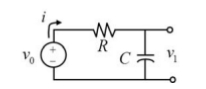
\includegraphics{foCircuit}
	\end{center}
	\caption{First Order Butterworth Filter (graphic taken from lab manual)}
	\label{fig:foCircuit}
\end{figure}

In analyzing the circuit we wish to find the voltage across the capacitor (this
can also be viewed as the output of the filter). First we apply the Kirchoff's
Voltage Law to the circuit:

\begin{align}
	V_0(t) &= V_R + V_C \label{eq:kvl}
	\\V_R &= iR \label{eq:ohmLaw}
	\\i &= C\frac{dV_C}{dt} \label{eq:capVoltage}
\end{align}
where $V_0$ is the voltage supply, $i$ is the current of the curcuit, $V_C$ is
the voltage across the capacitor, and $R$ and $C$ are the resistor and capacitor
values respectively. If we substitute \eqref{ohmLaw} and \eqref{capVoltage} into
\eqref{kvl} we get the following first order ODE:

\begin{align}
	RC\frac{dV_c}{dt} + V_c &= V_0(t) \label{eq:fo_ODE1}
\end{align}
If $V_0(t)$ is some step signal with magnitude voltage ($V_s$) then
\eqref{fo_ODE1} can be solved using the generic form (see equation $2.10$ in the
textbook):

\begin{align}
	V_C(t) = \left. V_s(1 - e^{\frac{-t}{\tau}}) \right| \tau = RC \label{eq:fo_Vc}
\end{align}
The constant $\tau$ is known as the time constant and has the property of.
$V_c(\tau) = (0.632)V_s$.

% subsection background (end)

\subsection{Analytical Time Constants} 
\label{sec:analytical_time_constants}

\tabref{fo_a_taus} shows the theoretical resistor and capacitor values along
with their theoretical time constant values and their corresponding experimental
contants.

\begin{table}[H]
  \begin{center}
		\caption{Analytical Time Constants}
		\label{tab:fo_a_taus}
		\begin{tabular}{ccccc}
      \\ \toprule
			\\ $R$ ($\Omega$) & $C$ (\dem{mF}) & $\tau_{\text{th}} = RC$ (\dem{s}) & $\tau_{\text{exp}} = RC$ (\dem{s}) & $\%Error$
      \\ \midrule
			\\  100 &  0.1061 &  1.061e-02 &  1.011e-02 &  -4.74
 \\  50 &  0.1061 &  5.305e-03 &  4.811e-03 &  -9.32
      \\ \bottomrule
    \end{tabular}
  \end{center}
\end{table}

\begin{figure}[H]
	\begin{center}
		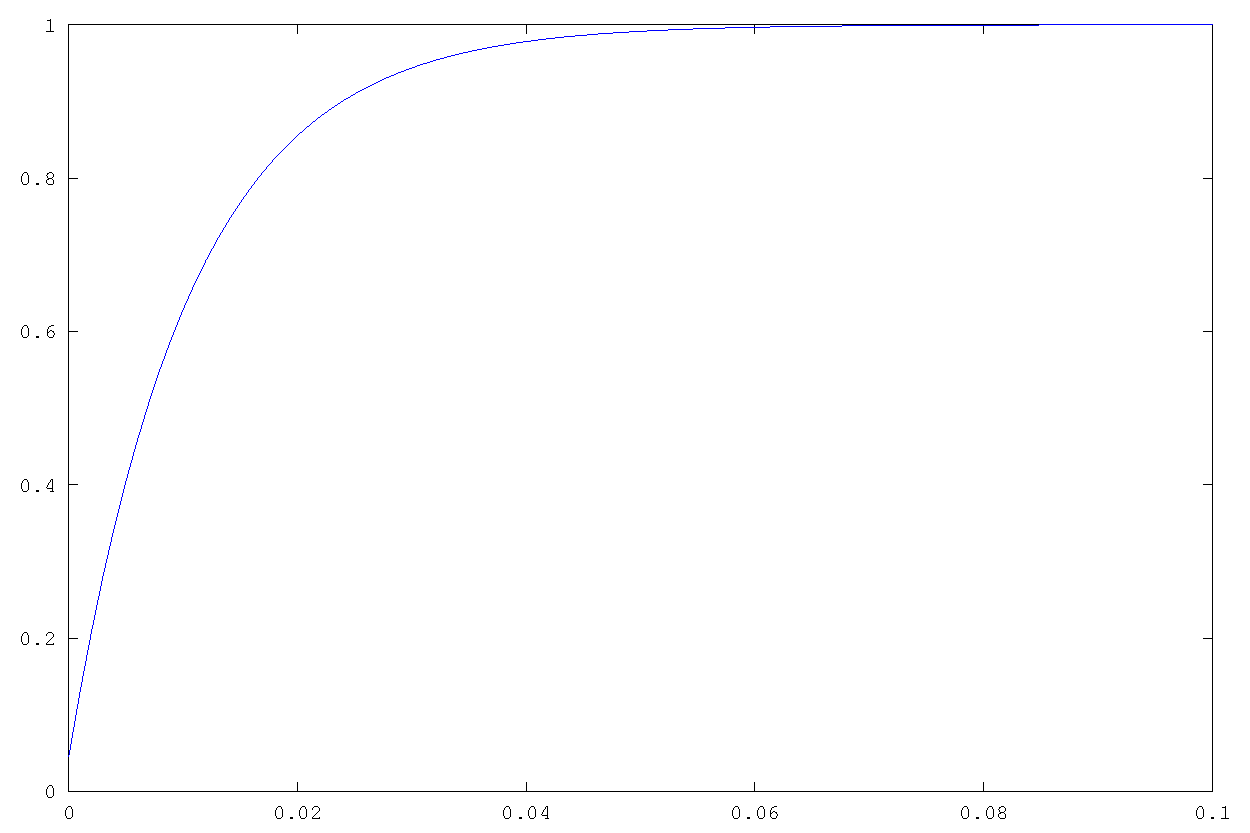
\includegraphics[width=\linewidth]{foAnalResponse.pdf}
	\end{center}
	\caption{First Order Butterworth Response}
	\label{fig:foGraph}
\end{figure}

% section analytical_time_constants (end)

% section first_order_differential_equations (end)

\end{document}
